\documentclass{article}


%%%%%%%%%%%%%%%%%%%%%%%%
%%%%%%%%%%%%%%%%%%%%%%%%
%%%%%%Packages
%%%%%%%%%%%%%%%%%%%%%%%%
%%%%%%%%%%%%%%%%%%%%%%%%

\usepackage{amsthm}
\usepackage{amsmath}
\usepackage{amssymb}
\usepackage[margin=1in]{geometry}
\usepackage{enumerate}
\usepackage{color}
\usepackage{graphicx}



%%%%%%%%%%%%%%%%%%%%%%%%
%%%%%%%%%%%%%%%%%%%%%%%%
%%%%%%amsthm settings
%%%%%%%%%%%%%%%%%%%%%%%%
%%%%%%%%%%%%%%%%%%%%%%%%

\theoremstyle{definition}
\newtheorem{problem}{Theorem}
\newtheorem{claim}{Claim}
\newtheorem{definition}{Definition}

%%%%%%%%%%%%%%%%%%%%%%%%
%%%%%%%%%%%%%%%%%%%%%%%%
%%%%%%Custom commands: mathbb
%%%%%%%%%%%%%%%%%%%%%%%%
%%%%%%%%%%%%%%%%%%%%%%%%

\newcommand{\A}{\mathbb A}
\newcommand{\C}{\mathbb{C}}
\newcommand{\D}{\mathbb{D}}
\newcommand{\E}{\mathbb{E}}
\newcommand{\F}{\mathbb{F}}
\newcommand{\N}{\mathbb{N}}
\renewcommand{\P}{\mathbb{P}}
\newcommand{\R}{\mathbb{R}}
\newcommand{\X}{\mathbb{X}}
\newcommand{\Z}{\mathbb{Z}}
\newcommand{\Q}{\mathbb{Q}}

%%%%%%%%%%%%%%%%%%%%%%%%
%%%%%%%%%%%%%%%%%%%%%%%%
%%%%%%Custom commands: greek
%%%%%%%%%%%%%%%%%%%%%%%%
%%%%%%%%%%%%%%%%%%%%%%%%

\renewcommand{\a}{\alpha}
\renewcommand{\b}{\beta}
\newcommand{\g}{\gamma}
\renewcommand{\d}{\delta}
\newcommand{\e}{\epsilon}
\renewcommand{\l}{\lambda}

\usepackage[utf8]{inputenc}

\title{Homework 1}
\author{Sean Eva}
\date{Math 4320}

\begin{document}

\maketitle

\begin{enumerate}
    \item [[\phantom{-}2]]
    
    \begin{enumerate}
        \item 
        
        Let $z \in \C$ such that $z = x + iy$ for some $x, y\in \R$. If we perform $iz = ix + i^2y = -y + ix$ and then $Re(iz) = -y$. Similarly, $Im(z) = y$ and therefore $-Im(z)= -y$. Thus, $Re(iz) = -Im(z) = -y$ as desired.
        
        \item
        
        Similarly to part a, $iz = -y = ix$ which implies that $Im(iz) = x$ and $Re(z) = x$. Thus $Im(iz) = Re(z) = x$ as desired.
        
    \end{enumerate}
    
    \item [[\phantom{-}10]]
    
    It will be useful to first recall the multiplication identity for reference purposes. $z_1 \dot z_2 = (x_1, y_1)(x_2, y_2) = (x_1x_2 - y_1y_2, y_1x_2 + x_1y_2) = (x_1x_2 - y_1y_2) + i(y_1x_2 + x_1y_2).$ We will now calculate $-(iy) = -((0, 1)(y, 0)) = -(0 - 0, 1y + 0) = (0, -y)$. Similarly, $(-i)y = (0, -1)(y, 0) = (0 - 0, -y + 0) = (0, -y).$ This would indicate what we desire that the additive inverse of a complex number $z = x + iy$ for $x,y\in \R$ can be written as $-z = -x -iy$. We will verify this.
    \begin{proof}
    Let $z\in \C$, that is to say that $z = x_1 + iy_1$ for some $x_1, y_1\in \R$ and we will denote a proposed additive inverse of a number as $(-z) = x_2 + iy_2$ for $x_2, y_2\in \R$. Then, by the definition of the additive inverse of a complex number, that $z + (-z) = (x_1 + iy_1) + (x_2 + iy_2) = 0 + 0i = 0$. We then have that $x_1 + x_2 = 0$ and $iy_1 + iy_2 = (y_1 + y_2)i = 0$ which we can extend to say that $y_1 + y_2 = 0$ since $i \neq 0.$ By the additive inverse rule of real numbers we then know that $x_1 + x_2 = 0$ and $y_1 + y_2 = 0$ implies that $x_2, y_2$ are the additive inverses of $x_1, y_1$ respectively. Therefore, we can denote them as $-x_1, -y_1$ which means that we can write $(-z) = -x_1 + i(-y_1) = -x_1 -  iy_1$. Therefore we can then explicitly write that the additive inverse of a complex number $z = x + iy$ as $-z = -x - iy.$
    \end{proof}
    
    \item [[\phantom{-}6]]
    
    \begin{proof}
    We can then write,
    \begin{align*}
        (\frac{z_1}{z_3})(\frac{z_2}{z_4}) &= z_1z_3^{-1}z_2z_4^{-1}\\
        &= z_1z_2z_3^{-1}z_4^{-1}\\
        &= (z_1z_2)(z_3^{-1}z_4^{-1})\\
        &= \frac{z_1z_2}{z_3z_4}.
    \end{align*}
    Therefore, we know that $(\frac{z_1}{z_3})(\frac{z_2}{z_4}) = \frac{z_1z_2}{z_3z_4}$ as desired.
    \end{proof}
    
    \item [[\phantom{-}3]]
    
    \begin{proof}
    Let $z_1, z_2, z_3, z_4 \in \C$. We know that $|z_3 + z_4| \geq ||z_3| - |z_4||$ which would imply that $\frac{Re(z_1 + z_2)}{|z_3 + z_4|} \leq \frac{Re(z_1 + z_2)}{||z_3| - |z_4||}$. Then we also know that $Re(z_1 + z_2) \leq |z_1 + z_2| \leq |z_1| + |z_2|$. Then we can extend our statement $\frac{Re(z_1 + z_2)}{|z_3 + z_4|} \leq \frac{Re(z_1 + z_2)}{||z_3| - |z_4||} \leq \frac{|z_1 + z_2|}{||z_3| - |z_4||} \leq \frac{|z_1| + |z_2|}{||z_3| - |z_4||}$. Thus we know that $\frac{Re(z_1 + z_2)}{|z_3 + z_4|} \leq \frac{|z_1| + |z_2|}{||z_3| - |z_4||}$ as desired.
    \end{proof}
    
    \item [[\phantom{-}4]]
    
    \begin{proof}
    Let $z\in \C$, then if we consider the original problem $\sqrt{2}|z| \geq |Re z| + |Im z|$ we could then say that $(\sqrt{2}|z|)^2 \geq (|Re z| + |Im z|)^2$. Then we can say $(\sqrt{2}|z|)^2 = 2|z|^2 = 2(\sqrt{x^2 + y^2})^2 = 2x^2 + 2y^2.$ Similarly, if we consider $(|Rez| + |Imz|)^2 = (|x| + |y|)^2 = x^2 + y^2 + 2|xy|$. Thus we can say that $(\sqrt{2}|z|)^2 - (|Re z| + |Im z|)^2 = 2x^2 + 2y^2 - x^2 - y^2 - 2|xy| = x^2 + y^2 - 2|xy| = (|x| - |y|)^2 \geq 0$. Therefore, this then implies that $\sqrt{2}|z| \geq |Re z| + |Im z|$ as desired.
    \end{proof}
    
    \item [[\phantom{-}8]]
    
    \begin{proof}
    Let $z_1, z_2 \in \C$ such that $z_1 = x_1 + iy_1$ and $z_2 = x_2 + iy_2$. Then we have that $z_1z_2 = (x_1x_2 - y_1y_2) + i(y_1x_2 + y_2x_1)$. Then it would follow that $|z_1z_2| = \sqrt{(x_1x_2 - y_1y_2)^2 + (y_1x_2 + y_2x_1)^2} = \sqrt{(x_1x_2)^2 - 2(x_1x_2y_1y_2) + (y_1y_2)^2 + (y_1x_2)^2 + (x_1y_2)^2 + 2(x_1x_2y_1y_2)} = \sqrt{(x_1x_2)^2 + (y_1y_2)^2 + (y_1x_2)^2 + (x_1y_2)^2} = \sqrt{x_1^2x_2^2 + y_1^2y_2^2 + y_1^2x_2^2 + x_1^2y_2^2} = \sqrt{(x_1^2 + y_1^2)(x_2^2+y_2^2)}$ as desired. It would then follow that $\sqrt{(x_1^2 + y_1^2)(x_2^2+y_2^2)} = \sqrt{(x_1^2 + y_1^2)}\sqrt{(x_2^2+y_2^2)} = |z_1||z_2|$ proving the identity.
    \end{proof}
    
    \item [[\phantom{-}2]]
    
    \begin{enumerate}
        \item 
        
        $Re(\bar{z} - i) = Re(\bar{z}) = Re(z) = 2$. Therefore if $z = x + iy$, then we know that $x = 2$. Therefore, we know that this is a vertical line at $x = 2.$
        
        \begin{figure}[h]
            \centering
            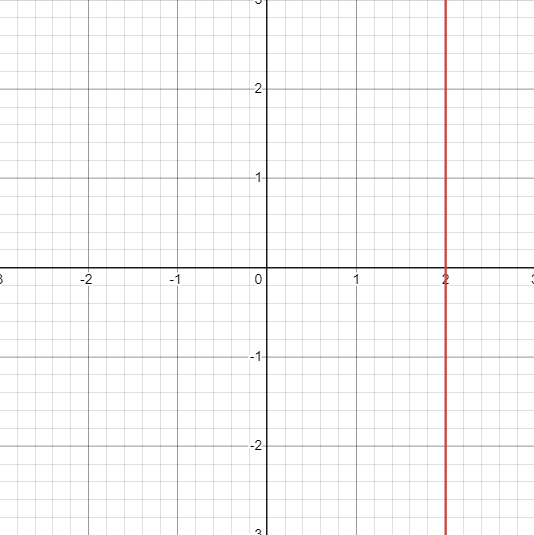
\includegraphics[width=0.4\textwidth]{figure_a.png}
        \end{figure} 
        
        \item
        
        We will first consider $|2\bar{z} + i| = 4$ and divide the whole equation by $2$ to get $|\bar{z} - (-\frac{i}{2})| = 2$. Literally, this means that the distance from $\bar{z}$ and $(-\frac{i}{2})$ is $2.$ If we then take the conjugate of this, we then know that the distance between $z$ and $\frac{i}{2}$ is $2$ which would imply that this is a circle of radius $2$ centered at $\frac{i}{2}$
        \\\\\\\\\\\\\\\\\\\\\\
        
        \begin{figure}[h]
            \centering
            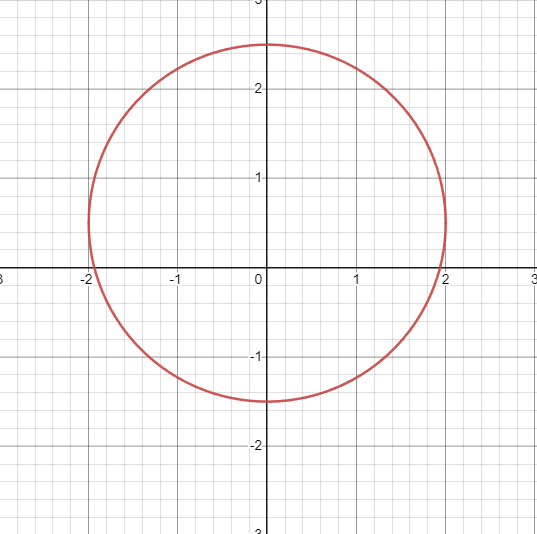
\includegraphics[width=0.4\textwidth]{figure_b.png}
        \end{figure} 
        
    \end{enumerate}
    
    \item [[\phantom{-}6]]
    
    \begin{enumerate}
        \item 
        
        \begin{proof}
        We know that $\bar{\frac{z_1}{z_2}} = \frac{\bar{z_1}}{\bar{z_2}}$. Then we know that $\bar{\frac{z_1}{z_2z_3}} = \frac{\bar{z}}{\bar{z_2z_3}}$. And since we also know that $\bar{z_1z_2} = \bar{z_1}\bar{z_2}$ then we can say that $\frac{\bar{z_1}}{\bar{z_2z_3}} = \frac{\bar{z_1}}{\bar{z_2}\bar{z_3}}$ as desired.
        \end{proof}
        
        \item
        
        \begin{proof}
        In a similar fashion to part a of this problem we have that $|\frac{z_1}{z_2}| = \frac{|z_1|}{|z_2|}$ and we have that $|z_1z_2| = |z_1||z_2|$. Therefore, we have that $|\frac{z_1}{z_2z_3}| = \frac{|z_1|}{|z_2z_3|} = \frac{|z_1|}{|z_2||z_3|}$ as desired.
        \end{proof}
        
    \end{enumerate}
    
    \item [[\phantom{-}11]]
    
    \begin{enumerate}
        \item 
        
        \begin{proof}
        Base Case: Let $n = 2$, then we have that $\bar{x_1 + x_2} = \bar{x_1} + \bar{x_2}$ as we know from the identity and then we know that the statement is true for $n = 2.$\\
        Inductive Step: Let the statement be true for $n = k$, that is to say that $\bar{x_1 + ... + x_k} = \bar{x_1} + ... + \bar{x_k}$. We now need to prove the statement for $n = k + 1$. We can then show $\bar{z_1 + ... + z_k + z_{k+1}}$ we will define $z = z_1 + ... + z_k$ and then show $\bar{z + z_{k + 1}} = \bar{z} + \bar{z_{k + 1}}$ and since we know that the statement is true for $n = k$ then we know that $\bar{z} = \bar{z_1 + ... + z_k} = \bar{z_1} + ... + \bar{z_k}$ which then means that $\bar{z_1 + ... + z_k + z_{k + 1}} = \bar{z_1} + ... + \bar{z_k} + \bar{z_{k + 1}}$. Thus, given the statement is true for $n = k$ and we were then able to show that the statement was true for $n = k + 1$ then we have proved that the statement is true for all $n = 2, 3, ...$ as desired.
        \end{proof}
        
        \item
        
        \begin{proof}
        Base Case: Let $n = 2$, then we have that $\bar{z_1z_2} = \bar{z_1}\bar{z_2}$ from the section and the statement is verified for $n = 2.$\\
        Inductive Step: Let the statement be true for $n = k$, that is to say that $\bar{x_1...x_k} = \bar{x_1}...\bar{x_k}$. We then want to show that the statement is true for $n = k + 1$. Consider if we set that $z = z_1...z_k$, we can then say that $\bar{zz_k} = \bar{z}\bar{z_k}$, and by the inductive hypothesis since we know that the statement is true for $n = k$, then we know that $\bar{z} = \bar{z_1...z_k} = \bar{z_1}...\bar{z_k}$ which allows us to say that $\bar{z_1...z_kz_{k+1}} = \bar{z_1}...\bar{z_k}\bar{z_{k + 1}}$ as desired. Therefore, since we knew that the statement was true for $n = k$, we were able to show that the statement was true for $n = k + 1$ and we know that the statement is further true for $n = 2, 3, ...$ as desired. 
        \end{proof}
        
    \end{enumerate}
    
    \item [[\phantom{-}1]]
    
    \begin{enumerate}
        \item 
        
        $z^{-1} = \frac{1+\sqrt{3}i}{-2} = \frac{-1}{2} + \frac{-\sqrt{3}}{2}i$ and that $z^{-1} = \frac{1}{r}e^{-i\theta}$. If we are only consider about finding $Arg(z)$ then we only need to find $\theta$. Therefore, we have that $\theta = \tan^{-1}(\frac{\frac{-\sqrt{3}}{2}}{\frac{-1}{2}}) = \tan^{-1}(\frac{\frac{\sqrt{3}}{2}}{\frac{1}{2}}) = \tan^{-1}(\sqrt{3})$ which we would then know the say that $\theta = -2\pi/3$ and since we know that the $\theta$ is negative, then we know that $\theta = 2\pi/3$
        
        \item
        
        We know that $z^6 = r^6e^{i6\pi}$ so then we know that $Arg(\sqrt{3} - i) = -\pi/6$ so then $6 * -\pi/6 = -\pi$. However, the principal argument $Arg (z)$ is defined $-\pi < \theta \leq \pi$ so then $Arg(z) = \pi.$
        
    \end{enumerate}
    
    \item [[\phantom{-}6]]
    
    \begin{proof}
    We already know from the section that $arg(z_1z_2) = arg(z_1) + arg(z_2)$; therefore, we need to show that when we take this sum for the $z_1, z_2$ in the problem statement that the resulting angle lies in the interval $(-\pi, \pi)$. Given that we know that $z_1$ and $z_2$ have positive real parts, then we know that their respective principal arguments are in the interval $(-\pi/2, \pi/2)$. Therefore, the sum of their principal arguments is in the interval $(-\pi, \pi)$ meaning that $Arg(z_1z_2) = Arg(z_1) + Arg(z_2)$ when $z_1, z_2$ have positive real components.
    \end{proof}
    
    \item [[\phantom{-}2]]
    
    We are going to note $z^3 = r^3e^{i3\theta}$. So if we set $z^3 = -8i = 8e^{i(-\pi/2)}$. Then we know that we can say that $z = (8)^{1/3}e^{i(-\pi/6)} = 2e^{i(-\pi/6)}$. So if we then convert the complex number to its standard form from the polar form, then we find that the cubed roots of $-8i$ are $\sqrt{3}-i, -\sqrt{3}-i, 2i.$
    
    \item [[\phantom{-}5]]
    
    \begin{proof}
    Let $z_0 = -4\sqrt{2} + 4\sqrt{2}i$, if we convert this to the polar form, we get that $z_0 = 8e^{i(-\pi/4)}$ or that $z_0 = 8e^{i(-\pi/4 + 2n\pi)}$ for $n \in \Z$. Then we know that the cube roots are given by $2e^{i(-\pi/12 + 2\pi/3)}$. Therefore, there are three solutions in a revolution, those being $2e^{i(-\pi/12)}, 2e^{i(7\pi/12)}, 2e^{i(15\pi/12)}$ which converted back into standard form are the other two solutions as desired.
    \end{proof}
    
\end{enumerate}

\end{document}